\documentclass[paper-main.tex]{subfiles}

\begin{document}

\begin{figure}
	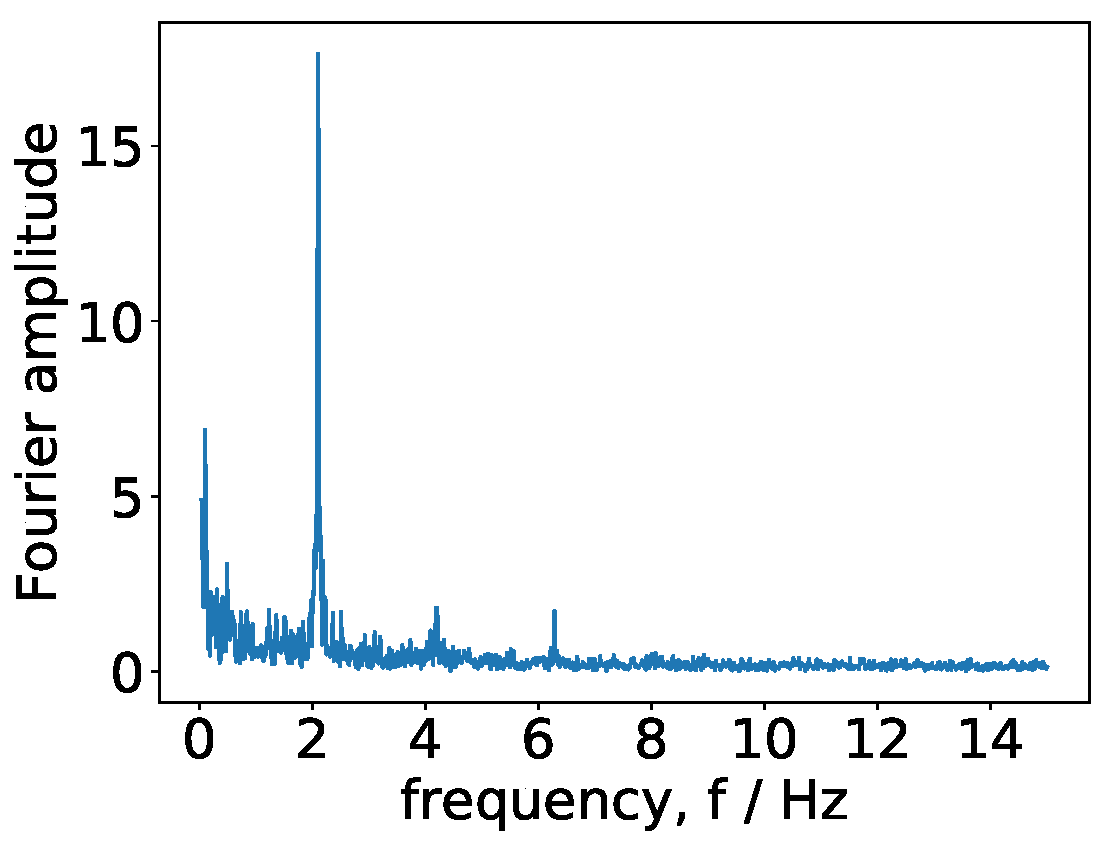
\includegraphics[width=.5\textwidth]{figures/webcam_spectrum_expt_4_0209.pdf}
	\caption{\label{fig:webcam_spectrum}
Recovery of a tone at a constant frequency: the Fourier amplitude of the intensity pattern against frequency.
The injected signal has a frequency of $2.09\,{\rm Hz}$, while the recovered signal peaks at $2.099\,{\rm Hz}$ and has an FWHM of $0.033\,{\rm Hz}$.
The plot also shows two harmonics at $4.19\,{\rm Hz}$ and $6.28\,{\rm Hz}$ with amplitudes $10.3 \%$ and $9.8 \%$ of the amplitude of the primary peak, respectively.
}	
\end{figure}



Continuous-wave searches look for nearly monochromatic signals~\cite{JKS:1998}. In this section, we consider a simple sinusoidal tone at a single, constant frequency. 


As described in Section~\ref{sec:ifo}, the audio signal is played through a speaker fixed to the back of M2 (see Fig.~\ref{fig:ifo_schematic_webcam}). 
The intensity of the interference pattern is measured at a single point on the screen, indicated by the pink star in Fig.~\ref{fig:interference_pattern}. 
The webcam records video in three color channels: red, blue, and green. 
We use the green channel as an approximation of the total intensity produced by the green laser.
The webcam samples at a rate of $30\, {\rm Hz}$, which limits the spectral content of observable signals to less than $15\,{\rm Hz}$, the Nyquist frequency. 



A tone with a frequency of $2.09\,{\rm Hz}$ is played through the speaker for one minute. 
The amplitude of the Fourier transform of the recovered signal is shown in Fig.~\ref{fig:webcam_spectrum}. The Discrete Fourier transform is calculated using the NumPy package for Python (see Appendix~\ref{app:code}).
We measured a peak amplitude at $2.099\,{\rm Hz}$ with a full width half maximum (FWHM) of $0.033\,{\rm Hz}$.
Two harmonics can also be seen at integer multiples of the peak frequency. 
The peaks at $4.19\,{\rm Hz}$ and $6.28\,{\rm Hz}$ have amplitudes of $0.103$ and $0.098$ as a fraction of the height of the main peak, respectively. They are likely due to the nonlinear response of the system discussed in Section~\ref{sec:ifo}.
Also, note that the noise appears to rise at lower frequencies, however the origin of this noise is not known. 


\end{document}
